% !TEX root = main.tex
\section{Calculation of global fluctuation
distributions\label{sec:4_calculation}}

The calculation of the fluctuation distributions from discrete dislocation configurations follows closely the analysis of section II. Some of the quantities left open are now given particular instantiation, and some of the continuous quantities must now be discretized. To begin with, the dislocation arrangement \(\mathcal{L}\) is now represented as the disjoint union of \(N_{\ell}\) discrete segments:
\begin{equation}
\mathcal{L}=\bigcup_{i = 0}^{N_{\ell}}\ell_{i}.
\end{equation}
The crystal space, which is a rectangular domain of size
\(\left( D_{1},D_{2},D_{3} \right)\), is then discretized into a
cubic mesh which divides the longest dimension of the crystal
(\(D_{1}\)) into \(N_{V}\) equal parts:
\begin{equation}
\boldsymbol{r}_{ijk}=L\left( i\hat{\boldsymbol{x}}+j\hat{\boldsymbol{y}} + k\hat{\boldsymbol{z}} \right).\qquad (i,j,k) \in \mathbb{N}^{3}
\end{equation}
for $\hat{\boldsymbol{x}}, \hat{\boldsymbol{y}}, \hat{\boldsymbol{z}}$ are the unit directions in space and the coarse-graining length is given as \(L \coloneqq D_{1}/N_{V}\). The
weight function by which the scalar dislocation density field is defined
at each point is chosen to be the cloud-in-cell function \cite{Birdsall1969}:
\begin{equation}
w_{L}\left( \boldsymbol{\Delta}\boldsymbol{r} \right)\coloneqq \begin{dcases}
\frac{1}{L^{3}}\prod_{I = 1}^{3}\left( 1 - \left| \frac{\Delta r_{I}}{L} \right| \right) & \text{if all } \left| \Delta r_{I} \right| \leq L \\
0 & \text{otherwise}.
\end{dcases}.
\end{equation}
The coarse-graining volume \(\Omega_{ijk}^{(L)}\) is thus the cube of
side length \(2L\) centered on the point \(\boldsymbol{r}_{ijk}\).

Focusing our attention on the collection of dislocation segments
surrounding a point
\(\Lambda_{ijk\ }^{(L)}=\mathcal{L}\cap\Omega_{ijk}^{(L)},\) we see
that we can assign to each segment \(\ell\) in this collection a
weight:
\begin{equation}
w_{\ell}^{(L)} = \int_{\ell}^{}{w_{L}\left( \boldsymbol{r -}\boldsymbol{r}_{ijk} \right)dl}.
\end{equation}
The density at this point is then given by the direct sum of these
weights:
\begin{equation}
\rho\left( \boldsymbol{r}_{ijk} \right)=\sum_{ \ell\in\Lambda_{ijk}^{(L)}}^{}w_{\ell}^{(L)}.
\end{equation}
Since each segment has a well-defined tangent direction
\({\hat{\boldsymbol{l}}}_{\ell}\) and thus orientation angle
\(\varphi_{\ell}\), we can
also define the average direction:
\begin{equation}
\beta_{1}^{(L)}\left( \boldsymbol{r}_{ijk} \right)e^{i{\overline{\varphi}}_{ijk}} = \frac{1}{\rho\left( \boldsymbol{r}_{ijk} \right)}\sum_{\ell \in \Lambda_{ijk}^{(L)}}^{}{w_{\ell}^{(L)}e^{i\varphi_{\ell}}}.
\end{equation}
This allows us to define the fluctuation angle
\(\delta_{\ell} = \varphi_{\ell} - {\overline{\varphi}}_{ijk}\)
for each segment.

These discrete definitions now allow us to define the local and global
fluctuation distributions. Obviously, we cannot consider the continuous
probability distributions. Instead, we will consider the probability that
the fluctuation directions fall in a sequence of \(N_{I}\) small
intervals which partition the unit circle:
\begin{subequations}
\begin{align}
    f_{ijk}^{(L)}\left( \delta \in I_{q} \right) &= \frac{1}{\rho\left( \boldsymbol{r}_{ijk} \right)}\sum_{\ell \in\Lambda_{ijk}^{(L)}}^{}{w_{\ell}^{(L)}1_{I_{q}}\left( \delta_{\ell} \right)},\\
     I_{q} &= \frac{2\pi}{N_{I}}\left\lbrack q - \frac{1}{2},q + \frac{1}{2} \right).
\end{align}
\end{subequations}
In the limit where \(N_{I} \rightarrow \infty\), this discretized
distribution converges to the fluctuation distribution function. We will
consider \(N_{I} = 360\), or single degree intervals. Regardless, the
global distribution can likewise be defined:
\begin{equation}
f^{(L)}\left( \delta \in I_{q} \right) = \frac{1}{\left| \mathcal{L} \right|}\sum_{ijk}^{}{\rho\left( \boldsymbol{r}_{ijk} \right)f_{ijk}^{(L)}\left( \delta \in I_{q} \right)}.
\end{equation}
Global averages over the angular fluctuations can be calculated either
by volume average of the local averages:
\begin{equation}\left\langle A(\delta) \right\rangle^{(L)} = \frac{1}{\left| \mathcal{L} \right|}\sum_{ijk}^{}{\sum_{\ell\in\Lambda_{ijk}^{(L)}}^{}{w_{\ell}^{(L)}A\left( \delta_{\ell} \right)}}\end{equation}
or by means of the discrete distribution function:
\begin{equation}\left\langle A(\delta) \right\rangle^{(L)} = \sum_{q = 1}^{2\pi}{f^{(L)}\left( \delta \in I_{q} \right)A\left( \frac{2\pi q}{N_{I}} \right)}.\end{equation}
Although the errors associated with the discretization of the angular
fluctuation space in the latter expression are small, we will still
prefer to utilize the former.

Now, given a discrete dislocation configuration, we can analyze all of
the angular statistics discussed at various coarse-graining lengths. The
particular discrete dislocation configurations used were obtained from a
set of 45 simulations performed in microMegas \cite{Devincre2011} which we have
utilized previously \cite{Anderson2021}. The simulations considered 4.40 x 4.87 x
\SI{5.74}{\micro\metre} domains of copper, seeded with random dipolar loops
resulting in an initial density of \SI{2}{\micro\metre^{-2}}. These domains were
then deformed at a {constant tensile strain rate along the [001] direction} to 0.3\% plastic strain. {Cross-slip was enabled at 300 K.} 
Dislocation configurations were extracted at strain increments of 0.075\%,
resulting in 180 configurations which will be analyzed according to the
framework just described.

{MicroMegas is a lattice-based discrete dislocation dynamics code, and so segments of a given slip system lie only along 8 discrete directions, which would obviously hinder analysis of orientation statistics. Because of this, glissile segment chains are resampled to segment midpoints to more smoothly represent the curved dislocation with straight segments. This also has the effect of allowing a broader range of segment orientations.}\footnote{{The resampled orientations are still limited to relatively low-order rational directions due to the lattice-based nature of the segment positions.}}{ For more information on this resampling, cf. chapter 5 of \cite{andersonStatisticalFoundationsLine2023}}.

\begin{figure}
    \centering
    \subfloat{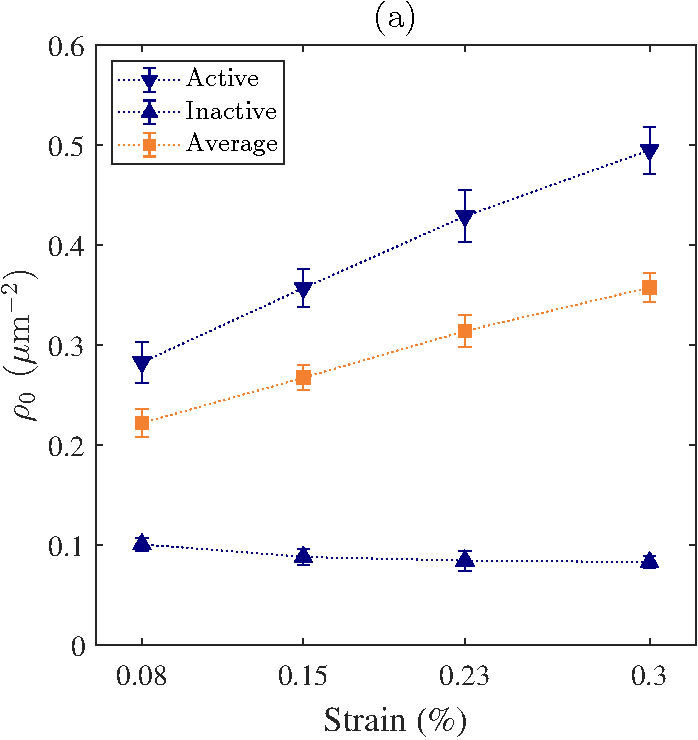
\includegraphics[height=2.5in]{Images/fig1a.pdf}}\\
    \subfloat{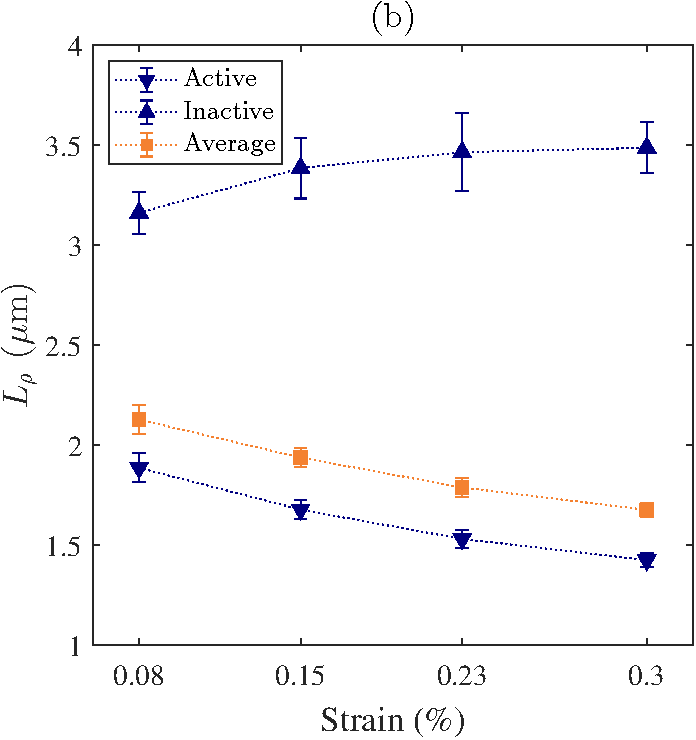
\includegraphics[height=2.5in]{Images/fig1b.pdf}}
    %\includegraphics[width=5in]{Images/fig1.pdf}
    \caption{Typical dislocation densities and mean dislocation spacing from the discrete dislocation configurations. Because of the asymmetry of dislocation multiplication and thus dislocation density on active and inactive slip systems, the calculations of the densities and corresponding average spacings are shown for the cases where these calculations are restricted to active and inactive slip systems as well as the unrestricted average. Error bars represent one standard deviation (over the set of 45 simulations).}
    \label{fig:SimulationStuff}
\end{figure}


The coarse-graining lengths which we will consider range from 71.5 nm to \SI{1.15}{\micro\metre}, corresponding to divisions of the longest edge of the crystal domain into 5 to 80 equal parts. However, we will not analyze these lengths as absolute distances. Rather, we will consider these coarse-graining lengths relative to the average dislocation spacing in the crystal. Because we treat only glissile dislocations and we treat every slip system as having its own fluctuation distribution, the relevant density for determining the average dislocation spacings (\(L_{\rho_{0}} = \left( \rho_{0} \right)^{- 1/2}\)) are:
\begin{equation}\rho_{0} = \frac{1}{12}\sum_{i = 1}^{12}\left| \mathcal{L}_{g}^{\lbrack\alpha\rbrack} \right|\end{equation}
where \(\left| \mathcal{L}_{g}^{\lbrack\alpha\rbrack} \right|\ \)is the total line length of glide dislocations on slip system \(\lbrack\alpha\rbrack\). The resulting dislocation densities and corresponding dislocation spacings are shown in \cref{fig:SimulationStuff}. Because each configuration has a distinct mean dislocation spacing, the absolute coarse-graining lengths will have various values when measured relative to these various dislocation spacings.

With all this in hand, we may now examine the global fluctuation distributions for various coarse-graining lengths. Also, we will compare the average characteristic sequence: 
\begin{equation} \beta_{n}^{(L)} = \left\langle e^{in\delta} \right\rangle^{(L)} \end{equation} 
across these coarse-graining lengths to determine regimes of coarse-graining length where the line bundle or maximum entropy closure relations [Eqs. (\ref{eq:LB1}-\ref{eq:LB2}, \ref{eq:ME1}-\ref{eq:ME2})] are appropriate.
